\begin{frame}[label=bragging]{Implementation (Hard case, unknown increment)}
  \begin{block}{Summary}
    \begin{itemize}
    \item Observe 64 outputs (4096 bits).
    \item Guess $k=$51--55 bits:
      \begin{itemize}
      \item $n=5$ successive rotations (6 bits each),
      \item $\ell=$ 11--13 least significant bits of \(S_0\) \textbf{and} \alert{$c$}.
      \end{itemize}
    \item Solve \(2^{k}\) instances of CVP in dimension 4 (Babai Rounding).
    \item Consistency Check.
    \end{itemize}
  \end{block}

  \begin{alertblock}{Caveat}
    \begin{itemize}
    \item Attack proved correct for $\ell=14$ (works fine for $\ell=13$).
    \item Succeeds with $p=0.66$ with $\ell=11$.
    \end{itemize}
  \end{alertblock}
  
  \begin{exampleblock}{Concretely...}
    \begin{itemize}
    \item $55$ CPU cycles per guess, 12.5k--20k CPU-hours in total.
    \end{itemize}
  \end{exampleblock}
\end{frame}

%%%%%%%%%%%%%%%%%%%%%%%%

\begin{frame}[label=bragging]{Doing it for Real}
  \begin{columns}
    \begin{column}[T]{3.5cm}
      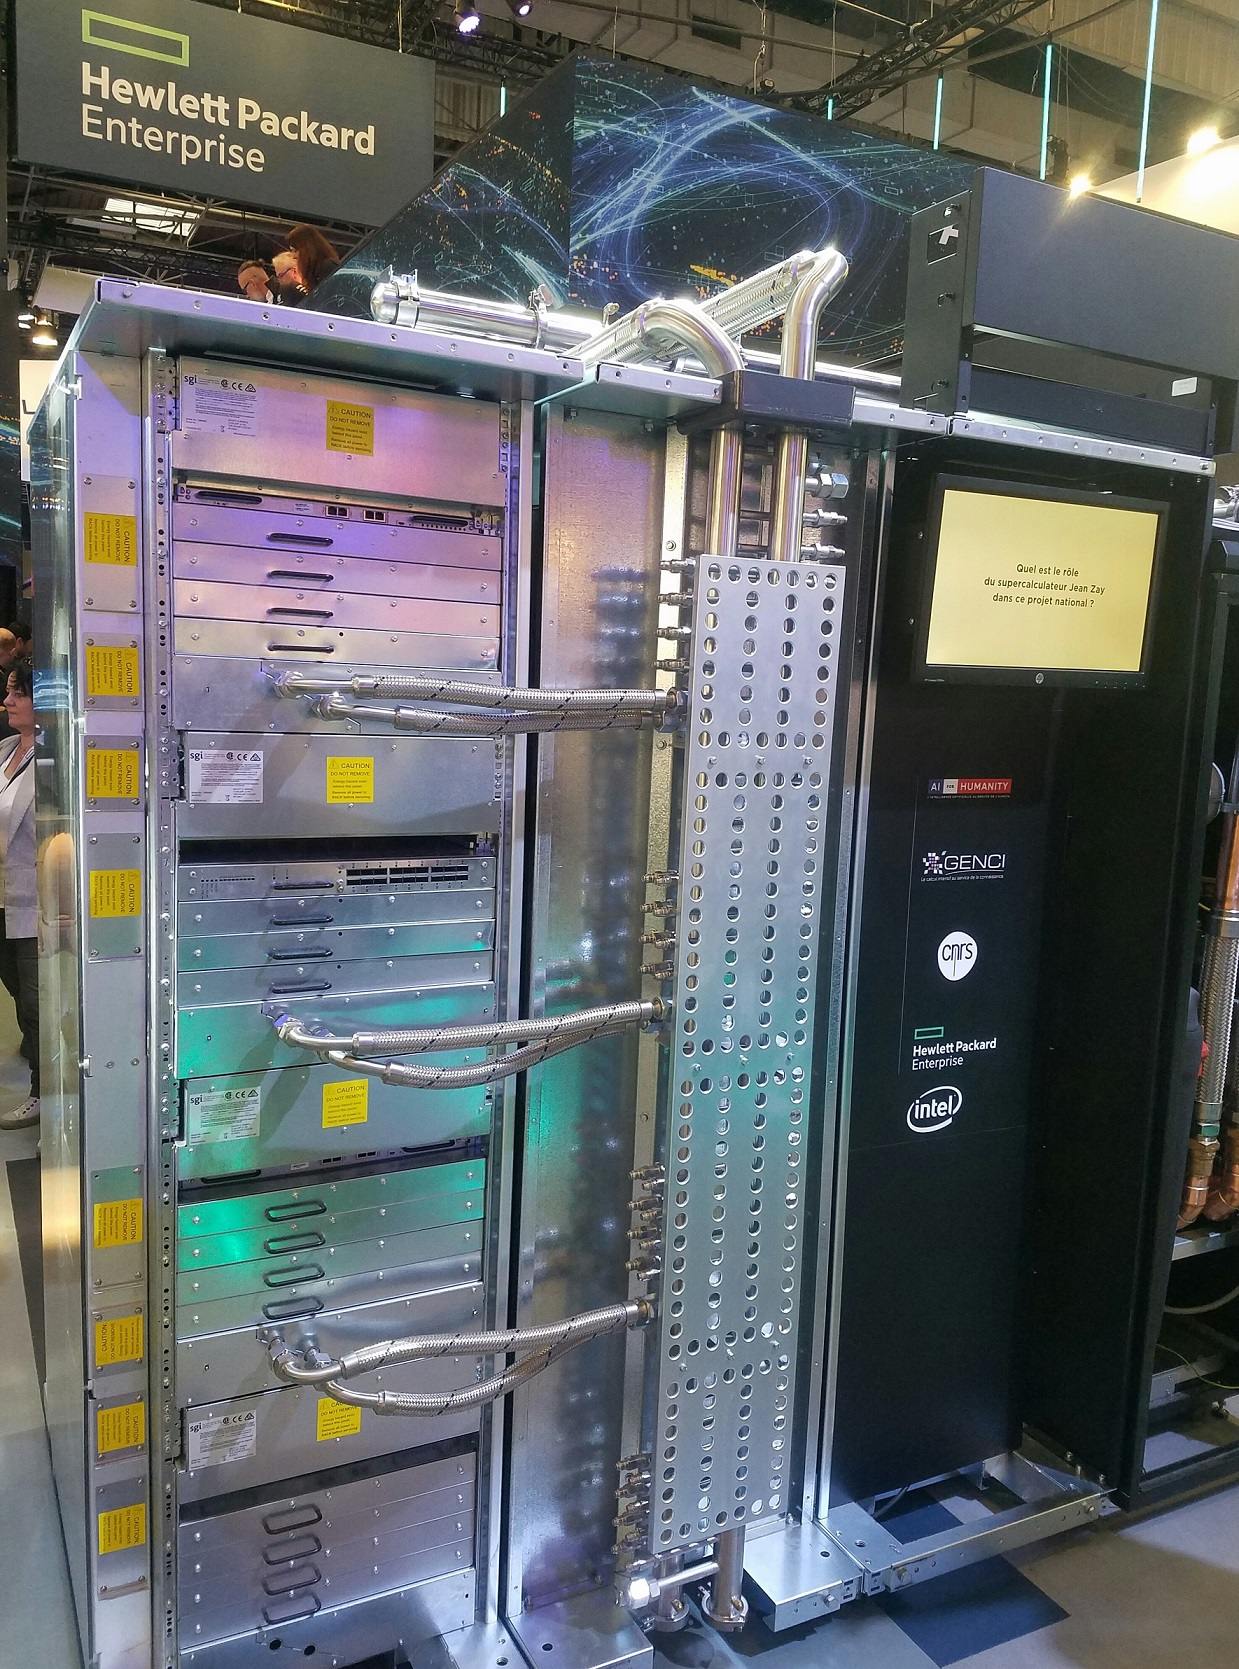
\includegraphics[height=0.6\textheight]{pictures/jean-zay.jpg}
    \end{column}
    \begin{column}[T]{6cm}
      \includegraphics[width=\textwidth]{pictures/jean_Zay.jpg}
    \end{column}
  \end{columns}
  
  \begin{itemize}
    \item Used 512 nodes
      \begin{itemize}
      \item 2$\times$20-core \textsf{Xeon Gold 6248 @ 2.5Ghz}
      \end{itemize}
    \item Running time: 35 minutes.
    \end{itemize}
  \end{frame}

%%%%%%%%%%%%%%%%%%%%%%%%%%%

  \begin{frame}{Conclusion}

  \begin{itemize}
    \item Reconstructing the seed for PCG is \textbf{practical}.
    \item PCG is \textbf{not} cryptographically secure (never claimed to be).
    \item \textbf{Don't} use \textsf{Numpy} to generate nonces...
    \end{itemize}
    
\end{frame}
  
  
%%% Local Variables:
%%% mode: latex
%%% TeX-master: "../main"
%%% End:
